\documentclass{beamer}
\usetheme{metropolis}
\setbeamersize{text margin left=1em, text margin right=1em}
\usepackage{amsmath, bm, enumitem}
\setlist[itemize]{noitemsep, topsep=1pt}

\usepackage{graphicx}
\usepackage{amsmath}
\usepackage{hyperref}

\title[AI Models]{Towards an Integrated Surveillance for Lassa fever: Evidence from the Predictive Modeling of Lassa fever Incidence in Nigeria.}
\author{Rebekah Lamai Gambo, Isah Charles Saidu, Yaknan John Gambo, Christian Rummel, Dominik Bohler, Sabine Dittrich}
\institute{..}
\date{\today}

\begin{document}

% Title slide
\begin{frame}
  \titlepage
\end{frame}

% Outline slide
\begin{frame}{Outline}
  \tableofcontents
\end{frame}

\section{Dataset: Overview}
\begin{frame}{Climate and Case Count Data}
\textbf{Data Overview:}
\begin{itemize}
    \item Weekly Lassa fever case counts for Bauchi, Edo, and Ondo states (Nigeria)
    \item Time period: January 2018 – December 2024
    \item Corresponding weekly climate data collected over the same period
\end{itemize}

\vspace{0.5em}
\textbf{Climate Variables (per week):}
\begin{itemize}
    \item Minimum Temperature
    \item Maximum Temperature
    \item Average Temperature
    \item Precipitation
    \item Precipitation Coverage
    \item Average Humidity
\end{itemize}
\end{frame}

\begin{frame}{Dataset: Plots}
  \includegraphics[width=\linewidth]{data_by_state.png}
\small
   Observations - The data appears to exhibit characteristics of a \textcolor{red}{stationary stochastic process}. 
\end{frame}

\begin{frame}{Dataset}
\textbf{Data  - Per State}
\begin{center}
    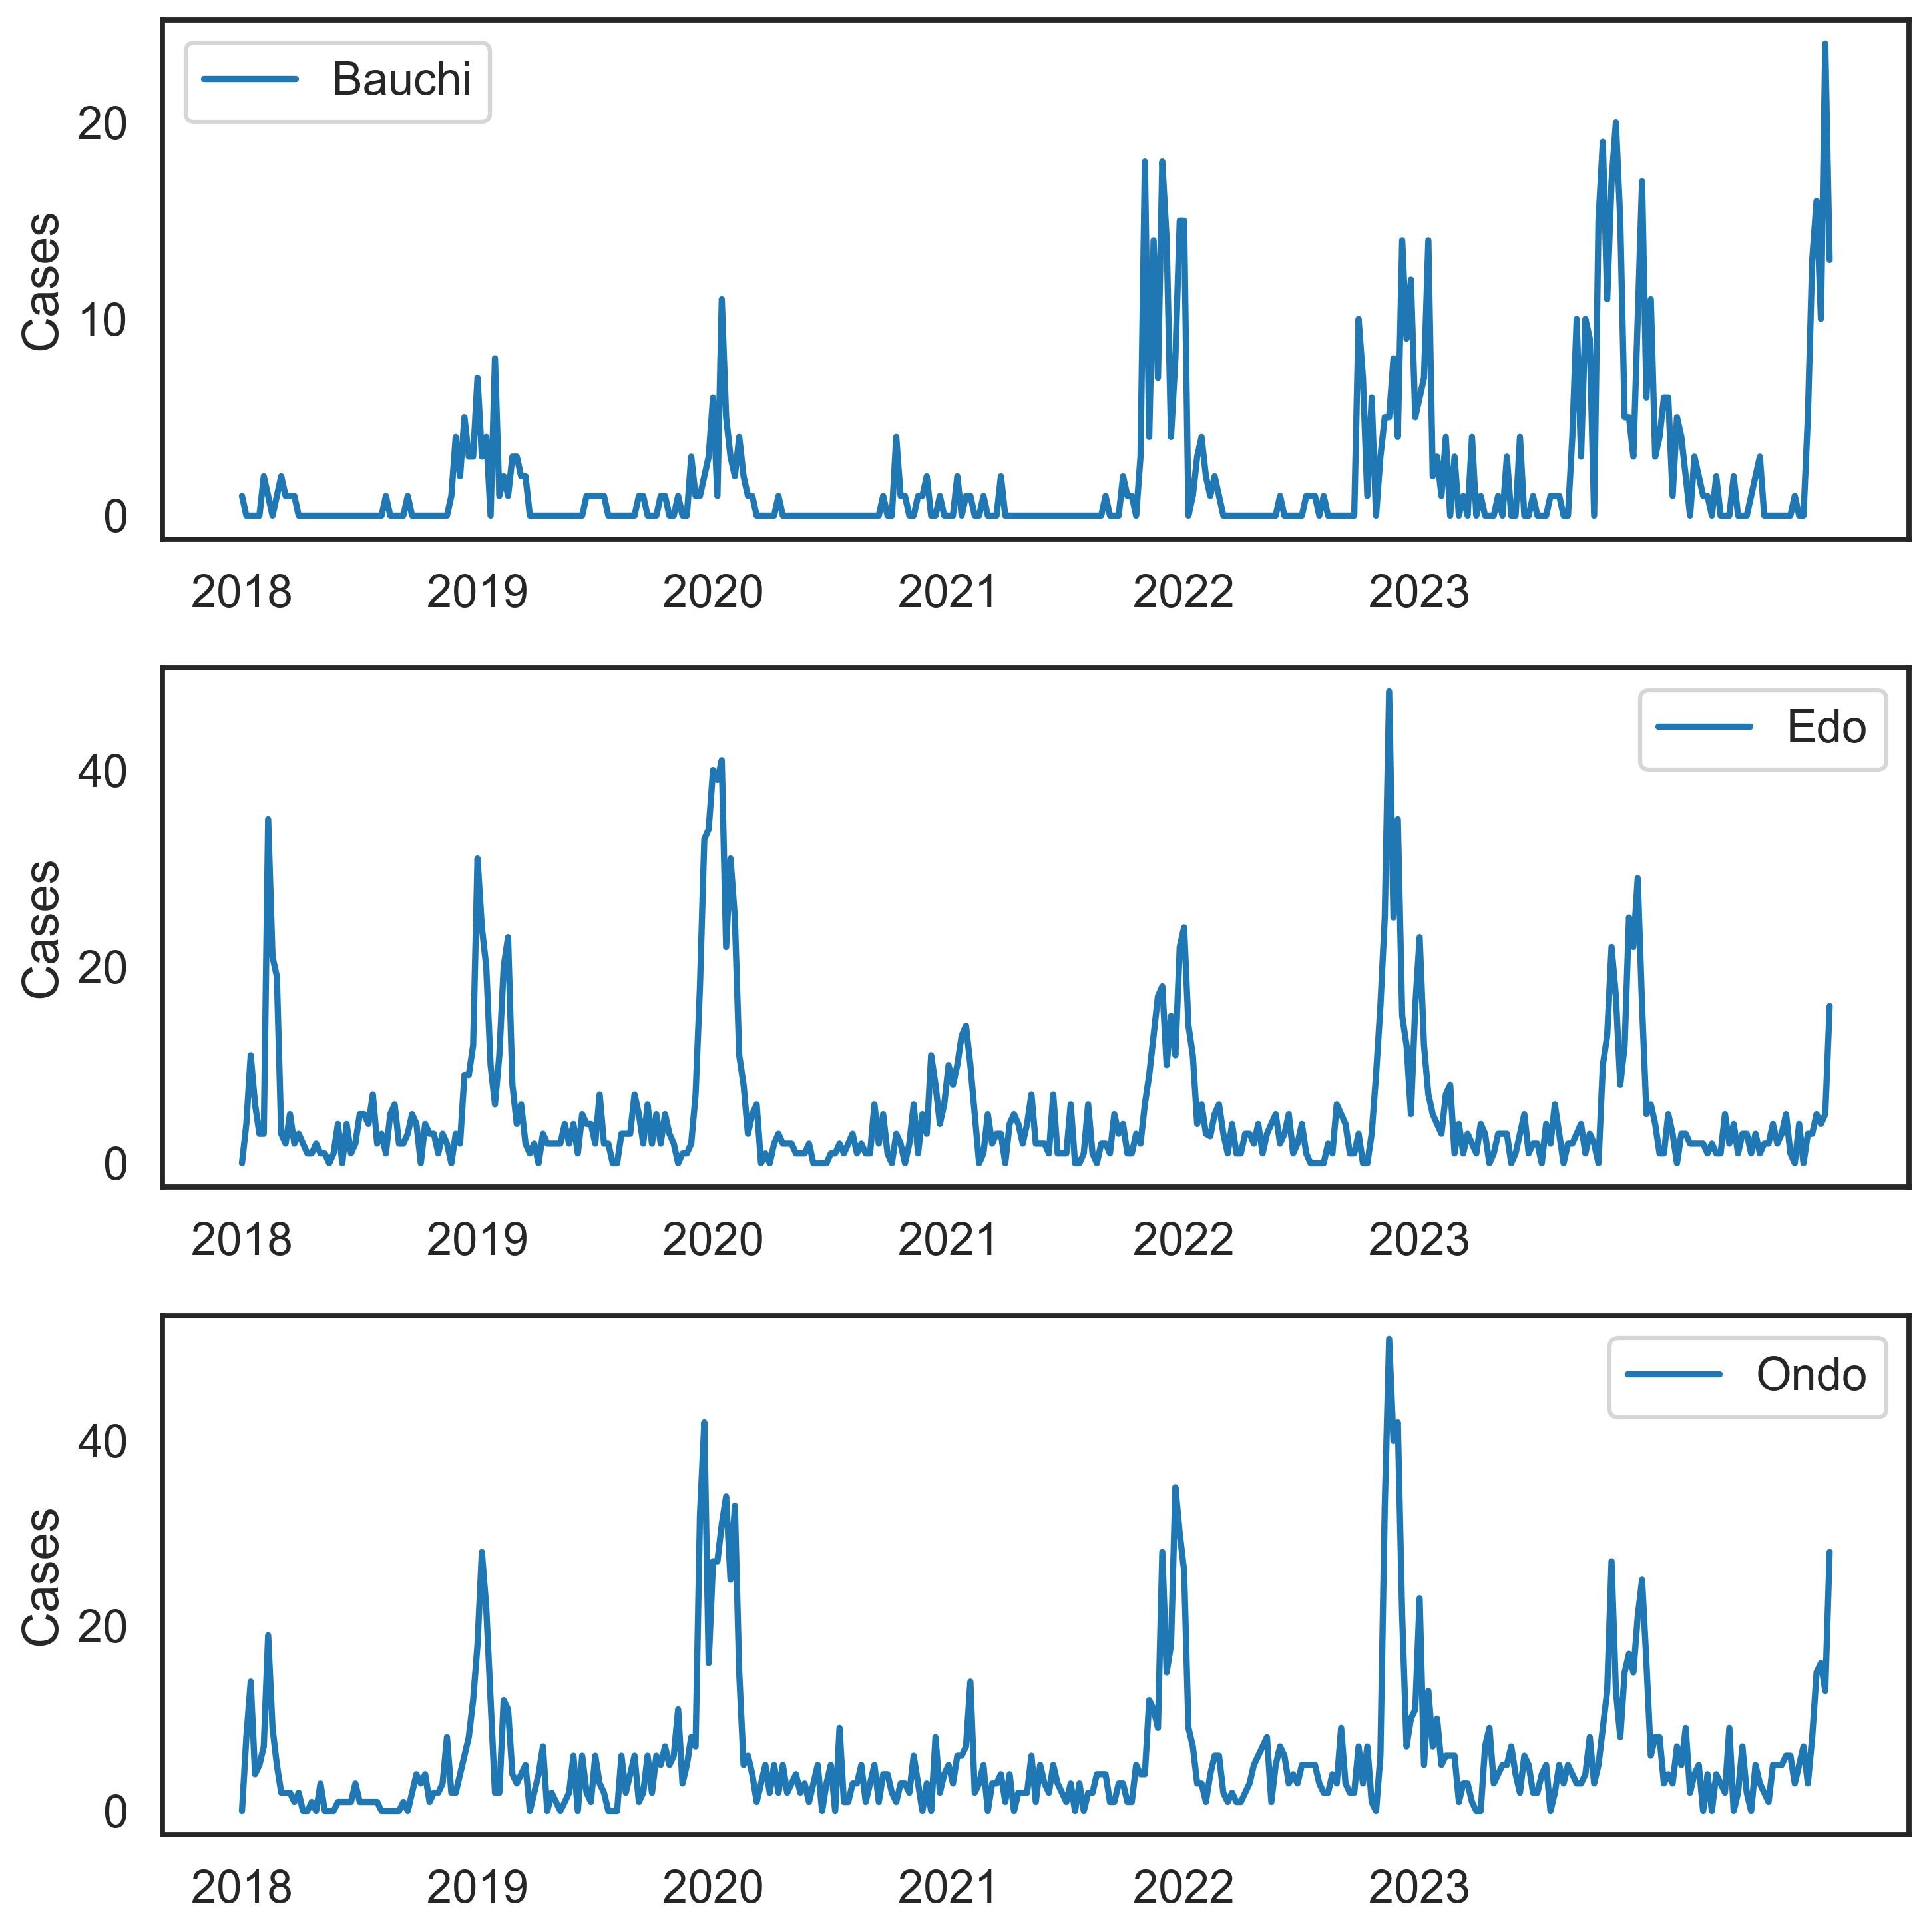
\includegraphics[scale = 0.3]{One_output_per_model/count_by_state.png}
\end{center}
\end{frame}


\begin{frame}{Data Split and Training Plan}

\textbf{Data Split:}
\begin{itemize}
    \item \textbf{Train:} 2018–2022 (per-state data)
    \item \textbf{Test:} 2023, 2024 (with prior context)
\end{itemize}

\vspace{0.5em}
\textbf{Modeling Strategies:}
\begin{itemize}
    \item LSTM
    \item MAR
\end{itemize}

\vspace{0.5em}
\textbf{Experiment Variants:}
\begin{itemize}
    \item \textbf{State-wise:} One model per state
    \begin{itemize}
        \item 7D input → 7D output (climate + cases)
        \item 7D input → 1D output ((climate , previous cases)→ cases)
    \end{itemize}
    \item \textbf{Unified:} One model across all states
\end{itemize}

\end{frame}



% Section 2: Types of AI Models
\section{Modeling Choices}

\subsection{Non-linear: Long short-term memory recurrent neural network (LSTM)}

\begin{frame}{Non-linear Model: Long Short-Term Memory (LSTM)}

\textbf{Prediction Variants:}
\begin{itemize}
    \item \textbf{Single-output (Lassa case count only):}
    \[
    y_t = f\left( \{\mathbf{y}_{t-i}\}_{i=1}^{4}; \mathbf{w} \right)
    \]
    
    \item \textbf{Multivariate output (case count + climate variables):}
    \[
    \mathbf{y}_t = f\left( \{\mathbf{y}_{t-i}\}_{i=1}^{4}; \mathbf{w} \right)
    \]
\end{itemize}

\vspace{0.5em}
\small
\textbf{Where:}
\begin{align*}
    & f \quad && \text{: LSTM prediction function} \\
    & y_t \in \mathbb{Z}^+ \quad && \text{: Predicted Lassa fever case count at time } t \\
    & \mathbf{x}_{t-i} \in \mathbb{R}^6 \quad && \text{: Climate variables at time } t-i \\
    & \mathbf{y}_t = (\mathbf{x}_t, y_t) \in \mathbb{R}^7 \quad && \text{: Full observation vector (climate + cases)} \\
    & t \quad && \text{: Discrete time step (e.g., week)} \\
    & \mathbf{w} \quad && \text{: Trainable parameters of the LSTM model}
\end{align*}

\end{frame}

\begin{frame}{LSTM Model: Training Loss Function}
\textbf{Given:} Training dataset (time index omitted for clarity)
\[
\mathcal{D} = \left\{ (\mathbf{x}_i, \mathbf{y}_i) \right\}_{i=1}^{n}, 
\quad \mathbf{x}_i \in \mathbb{R}^d,\quad \mathbf{y}_i \in \mathbb{R}^m
\]
\small
\textbf{Loss Function:}
\[
\mathcal{L}(\mathbf{w}) = 
\frac{1}{n} \sum_{i=1}^{n} \underbrace{\left\| f_{\mathbf{x}_i} - f(\mathbf{x}_i; \mathbf{w}) \right\|^2}_{\text{MSE loss (climate features)}}
+ \underbrace{ \sum_{i=1}^{n} \left[ f_y - y_i \log f_y \right]}_{\text{Poisson loss (case count)}}
+ \lambda \underbrace{\sum_{i=1}^{n} \left( \Delta f_y \right)^2}_{\text{Smoothness penalty}}
\]

\footnotesize
\textbf{Where:}
\begin{itemize}
    \item[] \( f(\mathbf{x}_i; \mathbf{w}) \): LSTM output for all targets
    \item[] \( f_y \): LSTM prediction of Lassa fever cases (scalar)
    \item[] \( f_{\mathbf{x}_i} \): LSTM prediction of climate variables (multi-output case)
    \item[] \( \Delta f_y = f_{y, t+1} - f_{y, t} \): First-order difference (temporal smoothness)
    \item[] \( \mathbf{w} \): Trainable LSTM parameters
    \item[] \( \lambda \): Smoothness regularization weight (e.g., 0.3)
\end{itemize}
\end{frame}



%%%%%%%%%%%%%%%%%%%%%%%%%%%%%%%%%%%%%%%%%%%
\subsubsection{One Model Per State - Climate + Cases Preditions}

% ----------------------------- Bauchi: All Variables -----------------------------
\begin{frame}{LSTM (Per-State Model) — Bauchi: Training Loss}
\textbf{Variant:} All Variables | One Model per State
\vspace{0.5em}

\textbf{Training Loss Curve}
\begin{center}
    \includegraphics[width=\linewidth]{Bauchi_train_viz.png}
\end{center}
\end{frame}

\begin{frame}{LSTM (Per-State Model) — Bauchi: Predictions}
\textbf{Variant:} All Variables | One Model per State
\vspace{0.5em}

\textbf{Training and Test Predictions}
\begin{center}
    \includegraphics[width=\linewidth]{Bauchi_predictions.png}
\end{center}
\end{frame}

% ----------------------------- Edo: All Variables -----------------------------
\begin{frame}{LSTM (Per-State Model) — Edo: Training Loss}
\textbf{Variant:} All Variables | One Model per State
\vspace{0.5em}

\textbf{Training Loss Curve}
\begin{center}
    \includegraphics[width=\linewidth]{Edo_train_viz.png}
\end{center}
\end{frame}

\begin{frame}{LSTM (Per-State Model) — Edo: Predictions}
\textbf{Variant:} All Variables | One Model per State
\vspace{0.5em}

\textbf{Training and Test Predictions}
\begin{center}
    \includegraphics[width=\linewidth]{Edo_predictions.png}
\end{center}
\end{frame}

% ----------------------------- Ondo: All Variables -----------------------------
\begin{frame}{LSTM (Per-State Model) — Ondo: Training Loss}
\textbf{Variant:} All Variables | One Model per State
\vspace{0.5em}

\textbf{Training Loss Curve}
\begin{center}
    \includegraphics[width=\linewidth]{Ondo_train_viz.png}
\end{center}
\end{frame}

\begin{frame}{LSTM (Per-State Model) — Ondo: Predictions}
\textbf{Variant:} All Variables | One Model per State
\vspace{0.5em}

\textbf{Training and Test Predictions}
\begin{center}
    \includegraphics[width=\linewidth]{Ondo_predictions.png}
\end{center}
\end{frame}

\subsubsection{One Model Per State - Cases Only Preditions}
% ----------------------------- One Output Models -----------------------------
% Bauchi
\begin{frame}{LSTM (Per-State, One-Output) — Bauchi: Training Loss}
\textbf{Variant:} One Output | One Model per State
\vspace{0.5em}

\textbf{Training Loss Curve}
\begin{center}
    \includegraphics[width=\linewidth]{One_output_per_model/Bauchi_train_viz.png}
\end{center}
\end{frame}

\begin{frame}{LSTM (Per-State, One-Output) — Bauchi: Predictions}
\textbf{Variant:} One Output | One Model per State
\vspace{0.5em}

\textbf{Training and Test Predictions}
\begin{center}
    \includegraphics[width=\linewidth]{One_output_per_model/Bauchi_predictions.png}
\end{center}
\end{frame}

% Edo
\begin{frame}{LSTM (Per-State, One-Output) — Edo: Training Loss}
\textbf{Variant:} One Output | One Model per State
\vspace{0.5em}

\textbf{Training Loss Curve}
\begin{center}
    \includegraphics[width=\linewidth]{One_output_per_model/Edo_train_viz.png}
\end{center}
\end{frame}

\begin{frame}{LSTM (Per-State, One-Output) — Edo: Predictions}
\textbf{Variant:} One Output | One Model per State
\vspace{0.5em}

\textbf{Training and Test Predictions}
\begin{center}
    \includegraphics[width=\linewidth]{One_output_per_model/Edo_predictions.png}
\end{center}
\end{frame}

% Ondo
\begin{frame}{LSTM (Per-State, One-Output) — Ondo: Training Loss}
\textbf{Variant:} One Output | One Model per State
\vspace{0.5em}

\textbf{Training Loss Curve}
\begin{center}
    \includegraphics[width=\linewidth]{One_output_per_model/Ondo_train_viz.png}
\end{center}
\end{frame}

\begin{frame}{LSTM (Per-State, One-Output) — Ondo: Predictions}
\textbf{Variant:} One Output | One Model per State
\vspace{0.5em}

\textbf{Training and Test Predictions}
\begin{center}
    \includegraphics[width=\linewidth]{One_output_per_model/Ondo_predictions.png}
\end{center}
\end{frame}

\subsubsection{LSTM Model Per State Model Comparison}
%%%%%%%%%%%%%%%%%%%%%%%%%%%%%%%%%%%%%%%%%%%%%%%%%%%%%%%%%%%%%%%%%%%%%
% Per state Model Comparison
%%%%%%%%%%%%%%%%%%%%%%%%%%%%%%%%%%%%%%%%%%%%%%%%%%%%%%%%%%%%%%%%%%
% Bauchi
\begin{frame}{Per-State Model Comparison: All vs One – Bauchi Predictions}
\textbf{All vs One – Output: Bauchi Predictions}
\begin{center}
    \includegraphics[width=\linewidth]{One_output_per_model/Bauchi_All_vs_One_predictions.png}
\end{center}
\end{frame}

% Edo
\begin{frame}{Per-State Model Comparison: All vs One – Edo Predictions}
\textbf{All vs One – Output: Edo Predictions}
\begin{center}
    \includegraphics[width=\linewidth]{One_output_per_model/Edo_All_vs_One_predictions.png}
\end{center}
\end{frame}

% Ondo
\begin{frame}{Per-State Model Comparison: All vs One – Ondo Predictions}
\textbf{All vs One – Output: Ondo Predictions}
\begin{center}
    \includegraphics[width=\linewidth]{One_output_per_model/Ondo_All_vs_One_predictions.png}
\end{center}
\end{frame}


\subsection{Linear: Mutivariate Autoregressive Model (Mar)}

\begin{frame}{MAR(4) Model for Climate and Lassa Fever Cases}
Let \( \mathbf{x}_t \in \mathbb{R}^7 \) be the multivariate time series defined by:
\[
\mathbf{x}_t = \begin{bmatrix}
x_t^{(1)} \\ x_t^{(2)} \\ \vdots \\ x_t^{(6)} \\ x_t^{(7)}
\end{bmatrix}
= \begin{bmatrix}
\text{climate}_t^{(1)} \\
\text{climate}_t^{(2)} \\
\vdots \\
\text{climate}_t^{(6)} \\
\text{lassa}_t
\end{bmatrix}
\]
The MAR(4) model is given by:
\[
\boxed{
\mathbf{x}_t  := f(\mathbf{x}_{t-1}; \mathbf{A})  = \sum_{k=1}^{4} A_k \mathbf{x}_{t-k} + \boldsymbol{\epsilon}_t, \quad \boldsymbol{\epsilon}_t \sim \mathcal{N}(\mathbf{0}, \Sigma)
}
\]

\small
\textbf{Lassa fever dynamics} (7th component):
\[
x_t^{(7)} = \sum_{k=1}^{4} \sum_{j=1}^{7} A_k^{(7,j)} x_{t-k}^{(j)} + \epsilon_t^{(7)} 
\]
\end{frame}


\begin{frame}{MAR(4) Model — One-Output Variant}
In the one-output version of the MAR(4) model, only Lassa fever cases are predicted based on the past values of climate variables:

\[
\boxed{
y_t = \sum_{k=1}^{4} A_k \mathbf{x}_{t-k} + \epsilon_t, \quad \epsilon_t \sim \mathcal{N}(0, \sigma^2)
}
\]

\smallskip
\textbf{Where:}
\begin{itemize}
    \item \( \mathbf{x}_t \in \mathbb{R}^7 \): vector of climate variables and the number of cases at time \( t \)
    \item \( A_k \in \mathbb{R}^{1 \times 7} \): autoregressive weight matrices
    \item \( y_t \): predicted number of Lassa fever cases at time \( t \)
\end{itemize}
\end{frame}

%%%%%%%%%%%%%%%%%%%%%%%%%%%%%%%%%%%%%%%%%%%%%%%%%%%%%%%%%%%%%%%%

\begin{frame}{Training Objective}

Let \( \mathcal{D} = \{(\mathbf{x}_i, \mathbf{y}_i)\}_{i=1}^{n} \) be the dataset, and let \( f(\mathbf{x}_i; \mathbf{A}) \) denote the model’s prediction.  
To reduce clutter, we omit the explicit time index \( t \).

\vspace{1em}

\textbf{Training Loss Function:}
\[
\boxed{
\mathcal{L}(\mathbf{A}) = \frac{1}{n} \sum_{i=1}^{n} \left\| \mathbf{x}_i - f(\mathbf{x}_i; \mathbf{A}) \right\|^2 
+ \lambda \sum_{j=1}^{d} \max(0, -\mathbf{y}_j)
}
\]

\vspace{1em}

\small
\textbf{Where:}
\begin{itemize}
    \item \( \mathbf{A} \): model coefficient matrices (e.g., MAR parameters)
    \item \( \max(0, -\mathbf{y}_j) \): regularization term penalizing negative outputs, enforcing \( \mathbf{y}_j \geq 0 \) for \( j = 1, \dots, d \)
    \item \( \lambda > 0 \): regularization hyperparameter
\end{itemize}

\end{frame}

\subsubsection{All Variable: One Mar Model Per State}


% ----------------------------- Mar Models-----------------------------
\begin{frame}{MAR (Per-State Model) — Bauchi: Training Loss}
\textbf{Variant:} All Variables | One Mar Model per State
\vspace{0.5em}

\textbf{Training Loss Curve}
\begin{center}
    \includegraphics[width=\linewidth]{MAR_model_per_state/Bauchi_state_MAR_One_Ouput_train_viz.png}
\end{center}
\end{frame}

\begin{frame}{MAR (Per-State Model) — Bauchi: Predictions}
\textbf{Variant:} All Variables | One MAR Model per State
\vspace{0.5em}

\textbf{Training and Test Predictions}
\begin{center}
    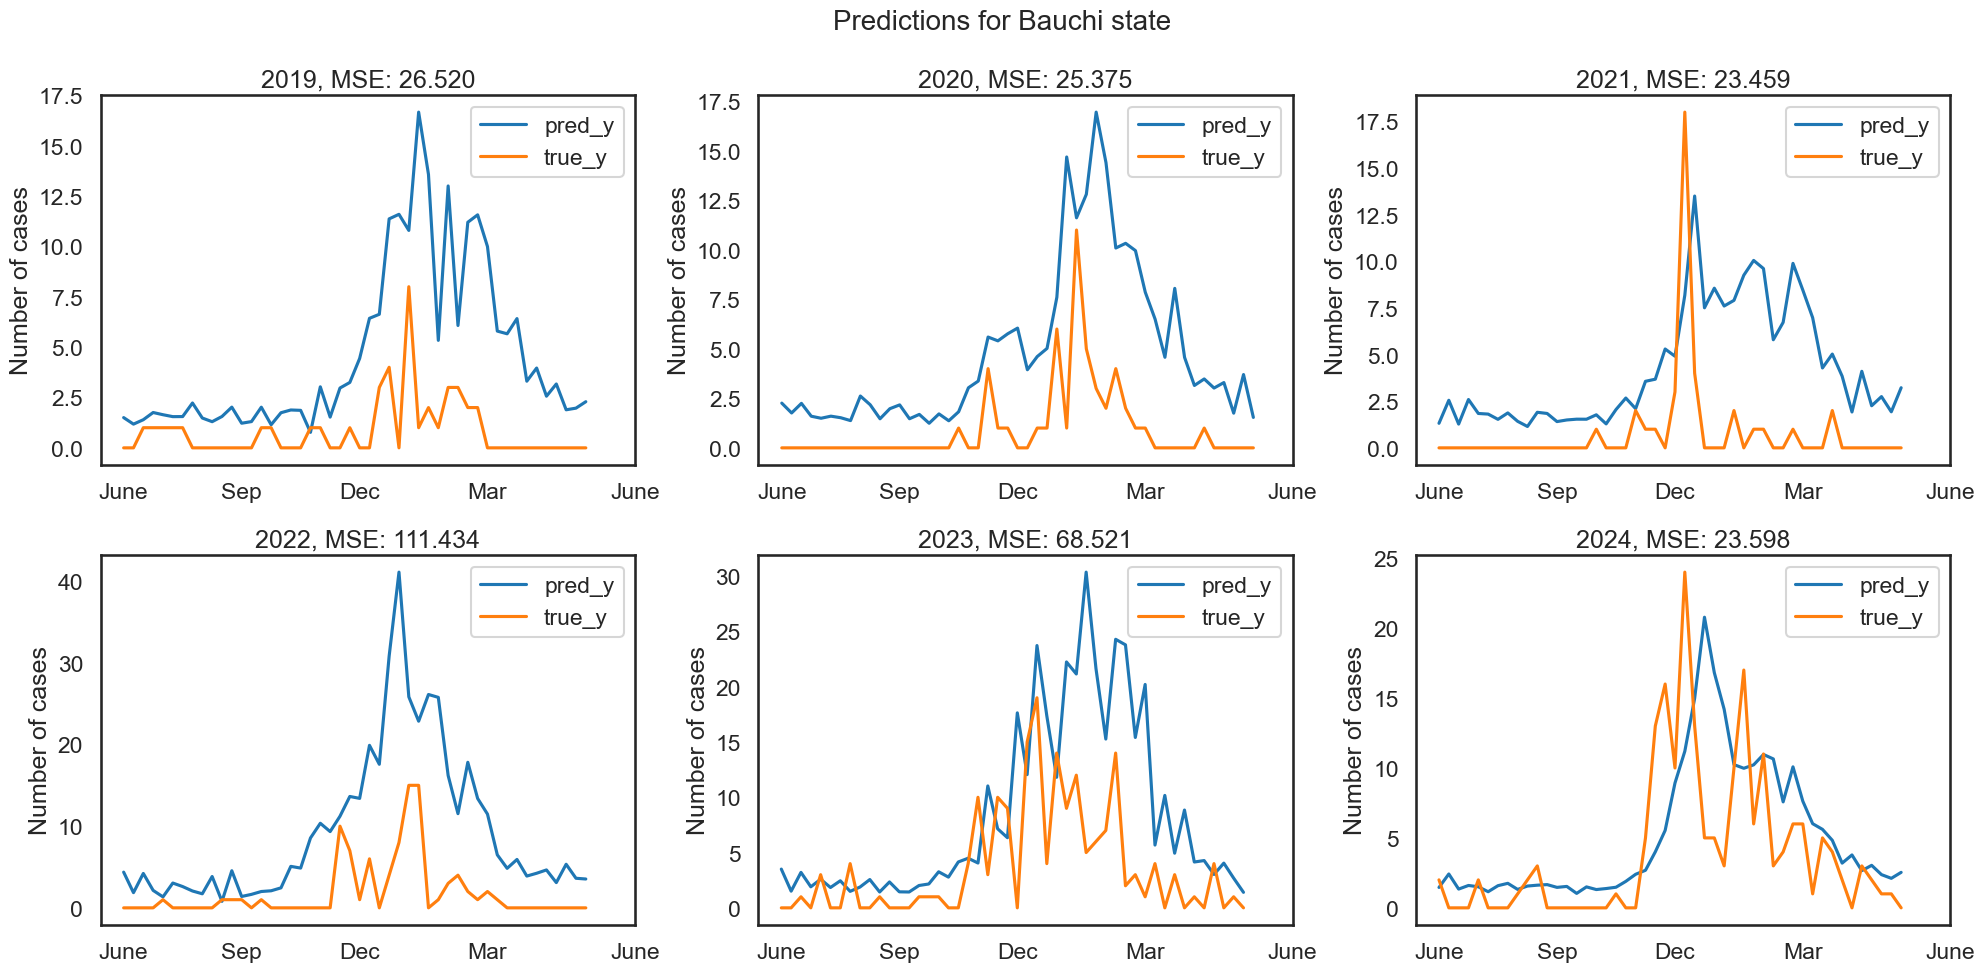
\includegraphics[width=\linewidth]{MAR_model_per_state/Bauchi_all_var_mar_predictions.png}
\end{center}
\end{frame}

% ----------------------------- Edo: All Variables -----------------------------
\begin{frame}{MAR (Per-State Model) — Edo: Training Loss}
\textbf{Variant:} All Variables | One MAR Model per State
\vspace{0.5em}

\textbf{Training Loss Curve}
\begin{center}
    \includegraphics[width=\linewidth]{MAR_model_per_state/Edo_state_MAR_One_Ouput_train_viz.png}
\end{center}
\end{frame}

\begin{frame}{MAR (Per-State Model) — Edo: Predictions}
\textbf{Variant:} All Variables | One MAR Model per State
\vspace{0.5em}

\textbf{Training and Test Predictions}
\begin{center}
    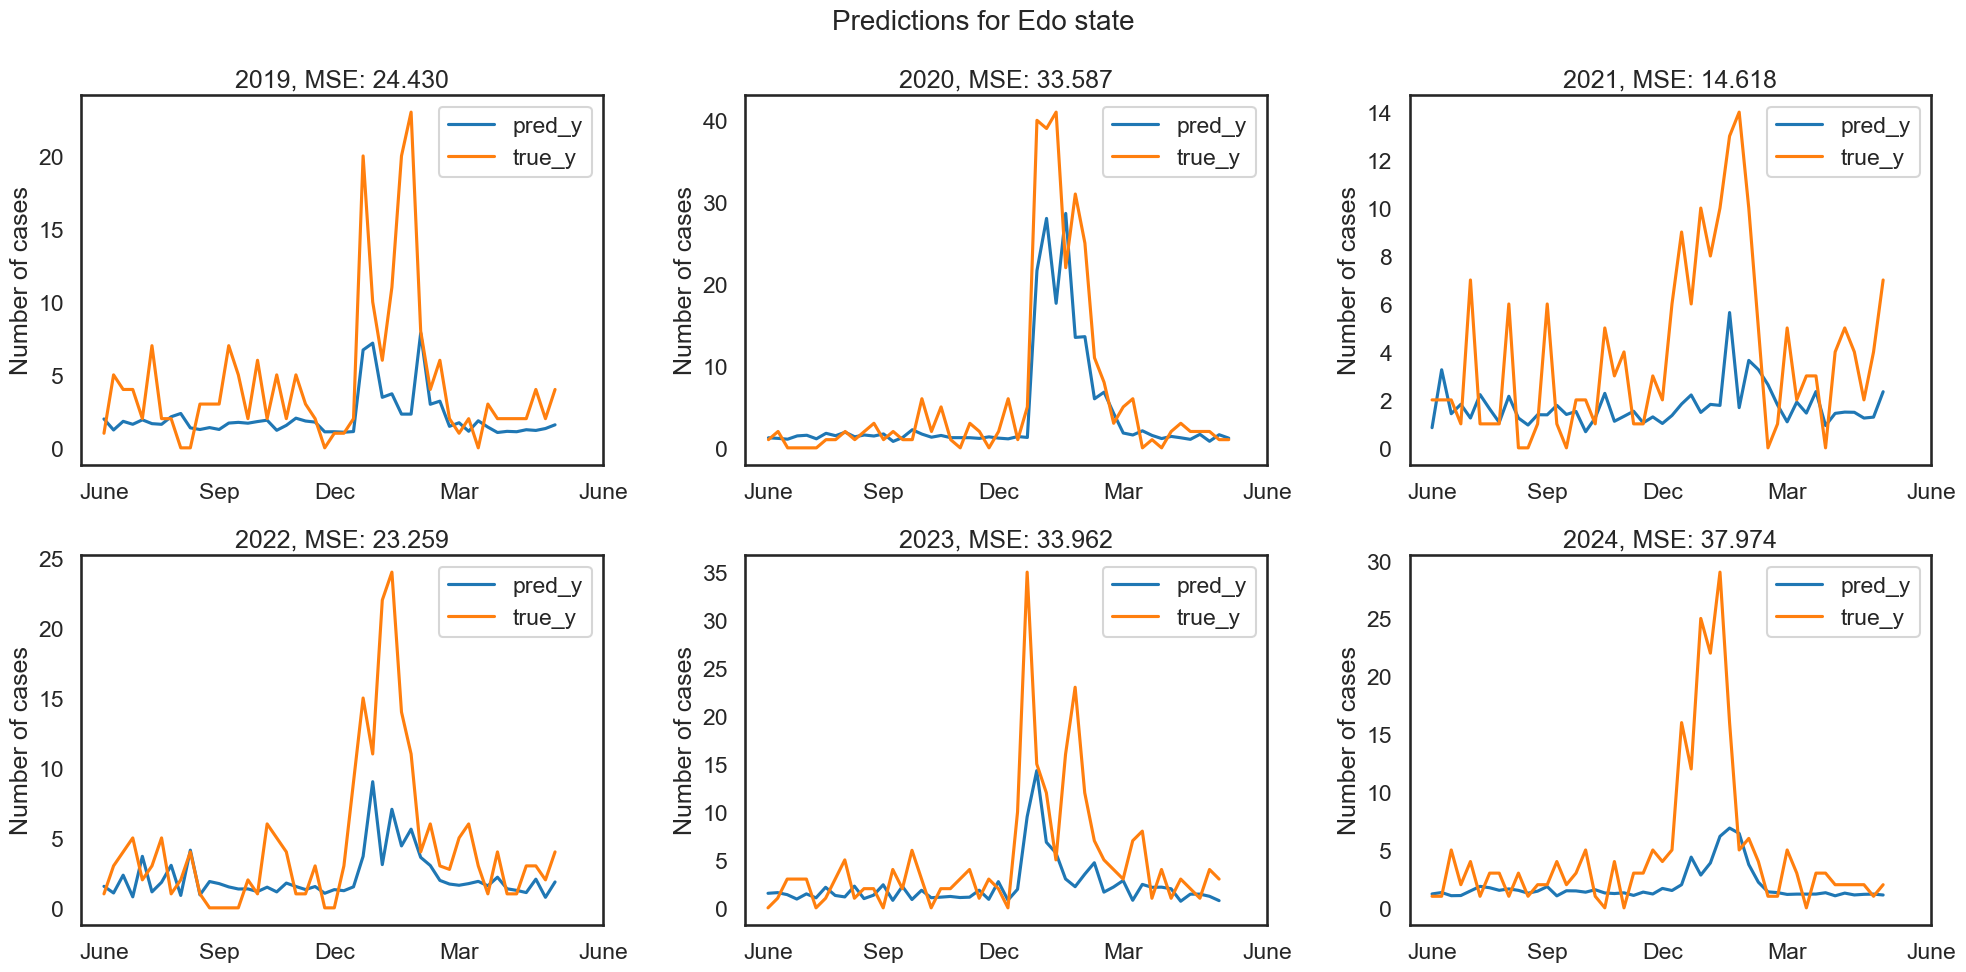
\includegraphics[width=\linewidth]{MAR_model_per_state/Edo_all_var_mar_predictions.png}
\end{center}
\end{frame}

% ----------------------------- Ondo: All Variables -----------------------------
\begin{frame}{LSTM (Per-State Model) — Ondo: Training Loss}
\textbf{Variant:} All Variables | One Model per State
\vspace{0.5em}

\textbf{Training Loss Curve}
\begin{center}
    \includegraphics[width=\linewidth]{MAR_model_per_state/Ondo_state_MAR_One_Ouput_train_viz.png}
\end{center}
\end{frame}

\begin{frame}{MAR (Per-State Model) — Ondo: Predictions}
\textbf{Variant:} All Variables | One MAR Model per State
\vspace{0.5em}

\textbf{Training and Test Predictions}
\begin{center}
    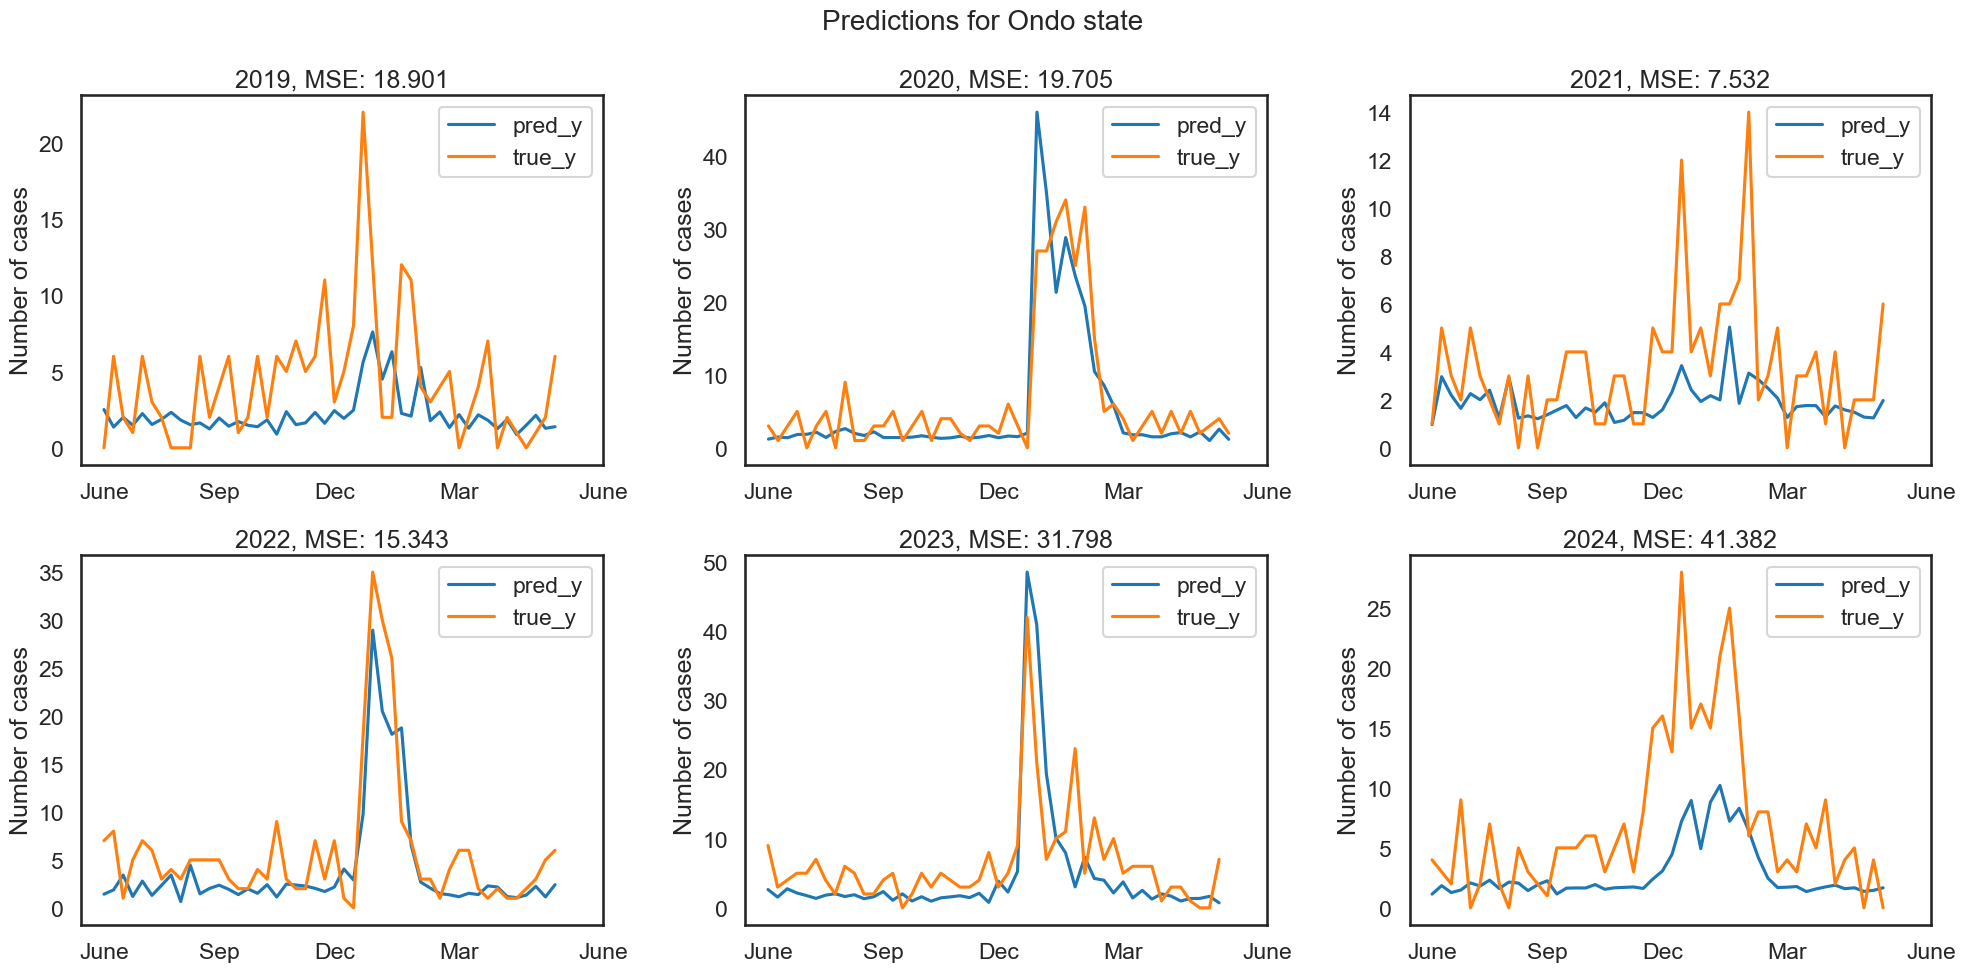
\includegraphics[width=\linewidth]{MAR_model_per_state/Ondo_all_var_mar_predictions.png}
\end{center}
\end{frame}
%
\subsubsection{One Mar Model Per State - Cases Only Preditions}
% ----------------------------- One Output Models -----------------------------
% Bauchi
\begin{frame}{Mar (Per-State, One-Output) — Bauchi: Training Loss}
\textbf{Variant:} One Output | One Model per State
\vspace{0.5em}

\textbf{Training Loss Curve}
\begin{center}
    \includegraphics[width=\linewidth]{MAR_model_Per_State_One_Output/Bauchi_state_MAR_One_Ouput_train_viz.png}
\end{center}
\end{frame}

\begin{frame}{Mar (Per-State, One-Output) — Bauchi: Predictions}
\textbf{Variant:} One Output | One Mar Model per State
\vspace{0.5em}

\textbf{Training and Test Predictions}
\begin{center}
    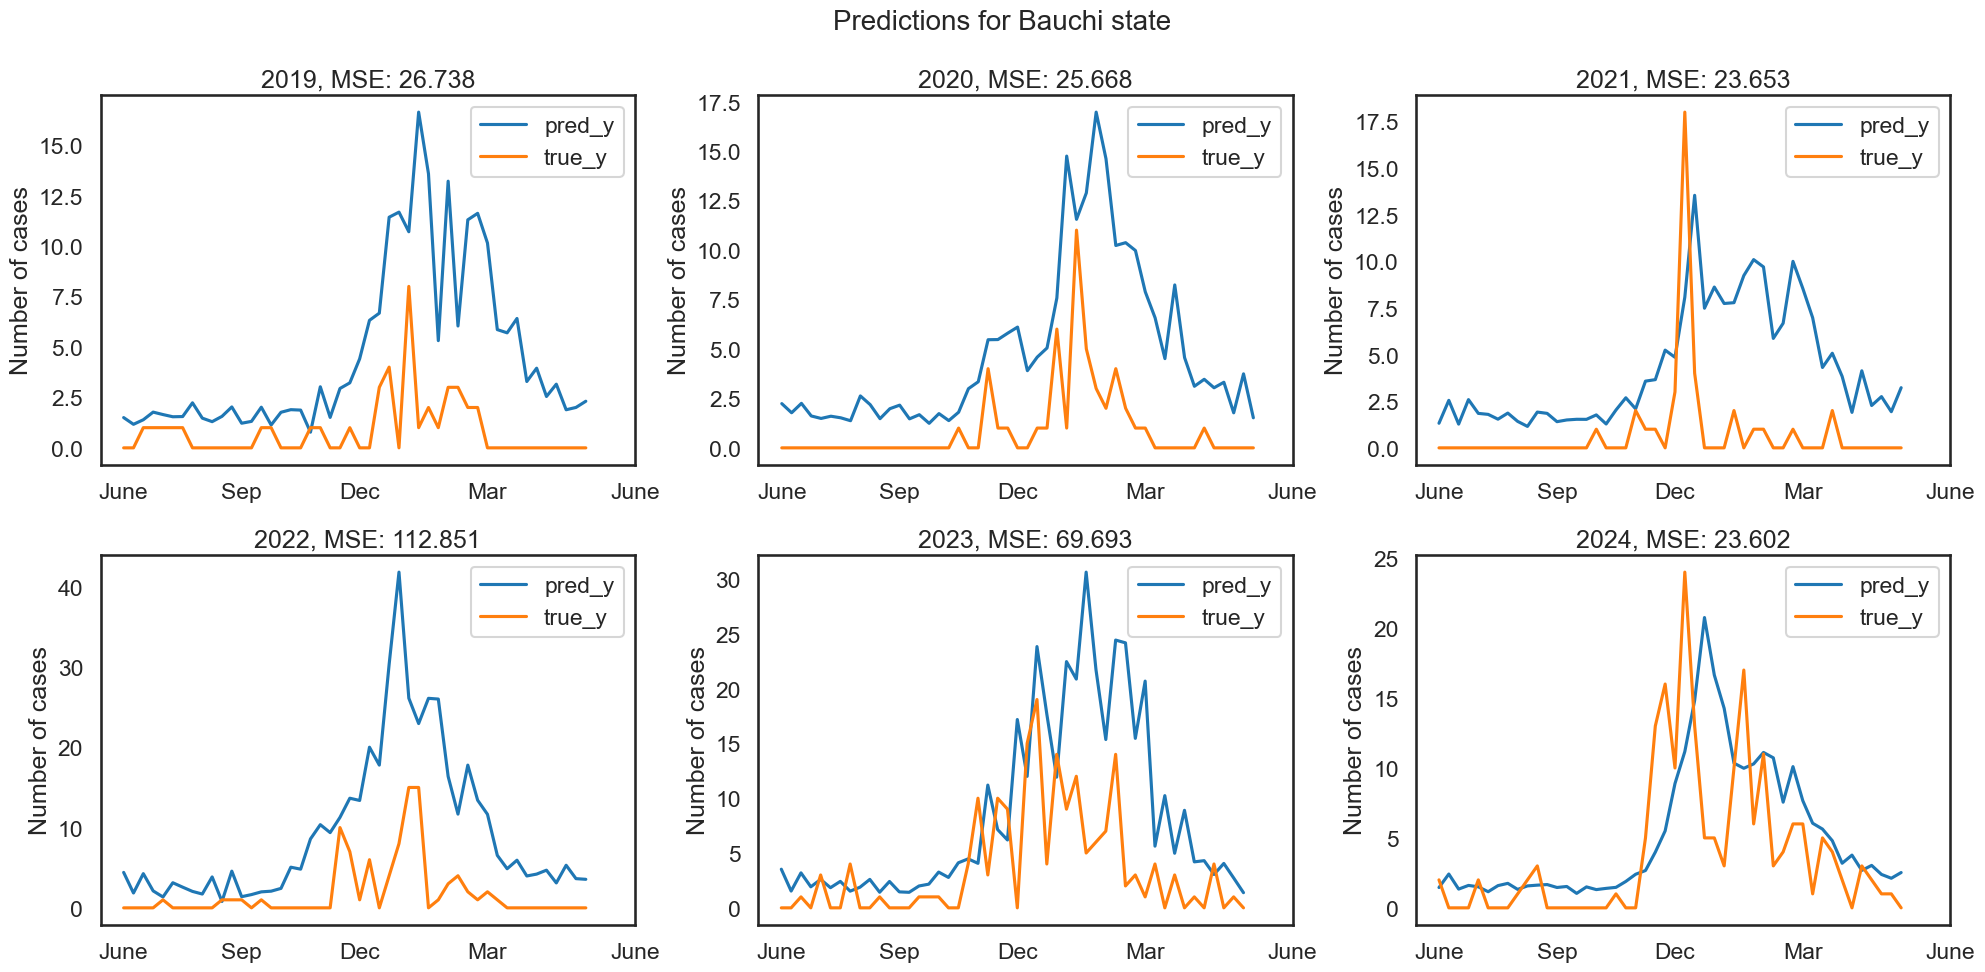
\includegraphics[width=\linewidth]{MAR_model_Per_State_One_Output/Bauchi_mar_predictions.png}
\end{center}
\end{frame}
%
% Edo
\begin{frame}{Mar (Per-State, One-Output) — Edo: Training Loss}
\textbf{Variant:} One Output | One Mar Model per State
\vspace{0.5em}

\textbf{Training Loss Curve}
\begin{center}
    \includegraphics[width=\linewidth]{MAR_model_Per_State_One_Output/Edo_state_MAR_One_Ouput_train_viz.png}
\end{center}
\end{frame}

\begin{frame}{Mar (Per-State, One-Output) — Edo: Predictions}
\textbf{Variant:} One Output | One Mar Model per State
\vspace{0.5em}

\textbf{Training and Test Predictions}
\begin{center}
    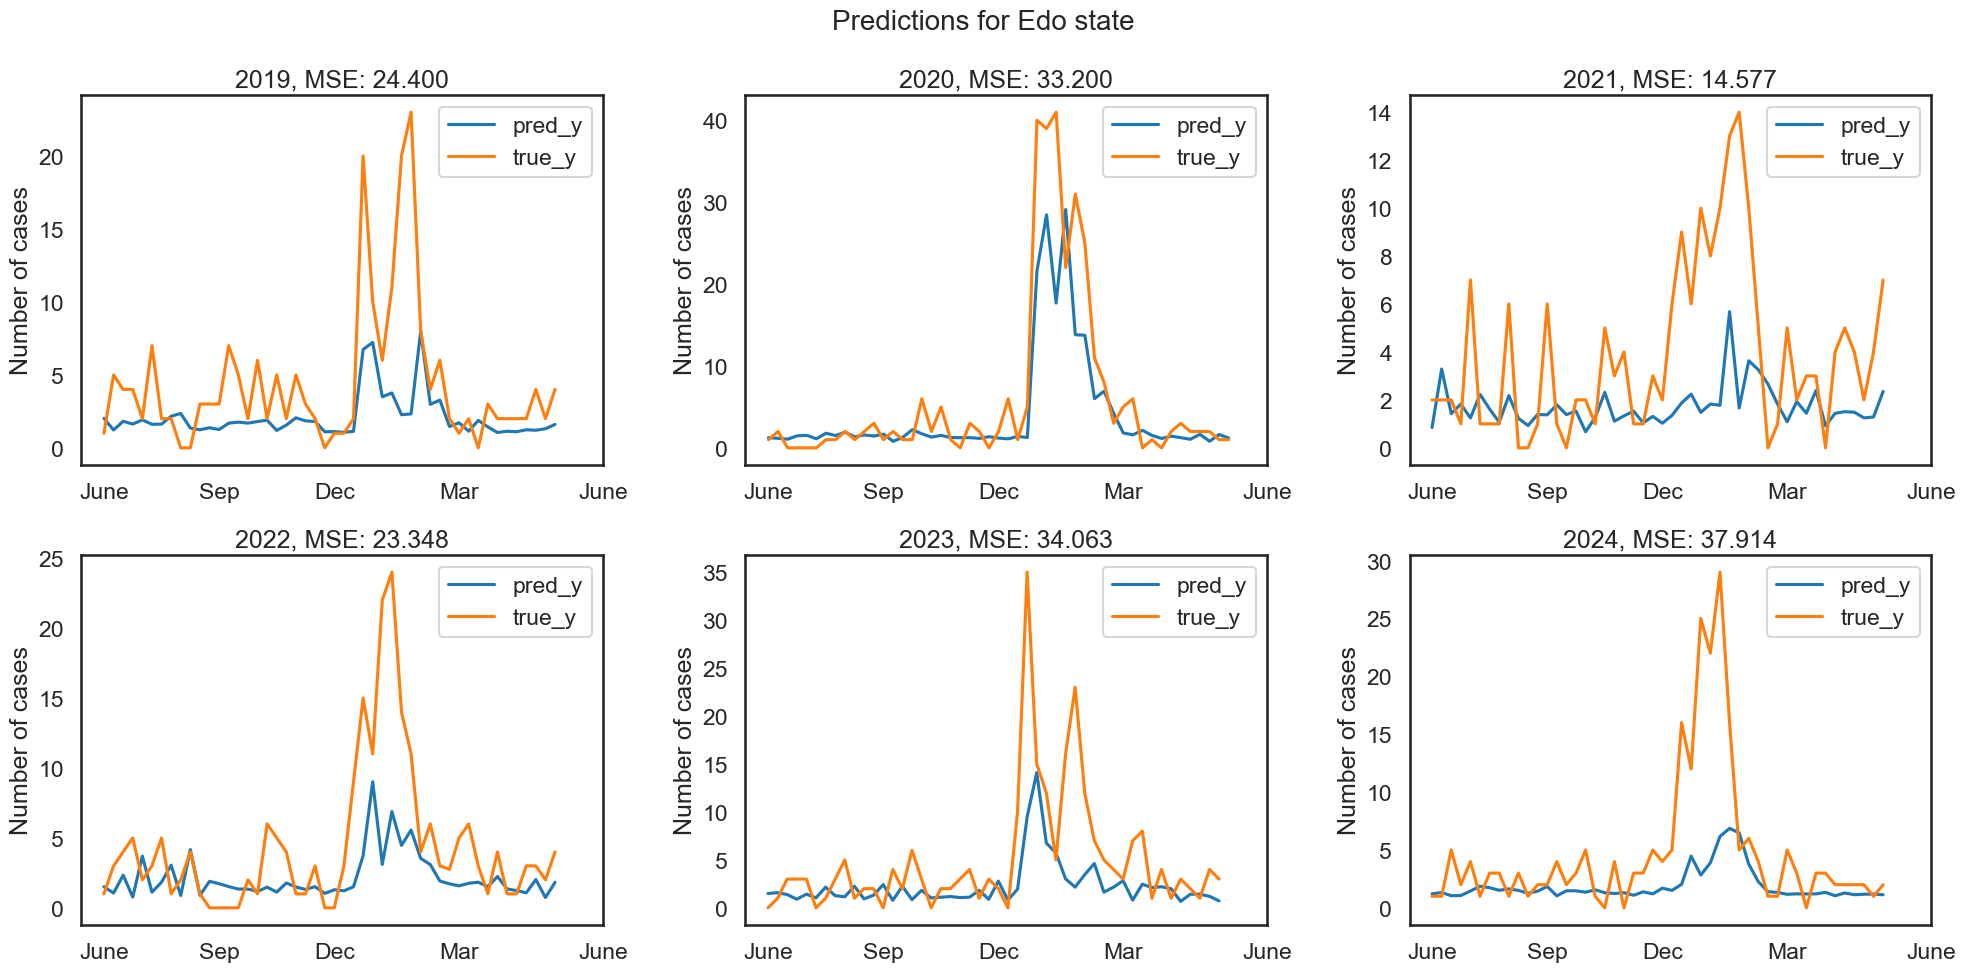
\includegraphics[width=\linewidth]{MAR_model_Per_State_One_Output/Edo_mar_predictions.png}
\end{center}
\end{frame}

% Ondo
\begin{frame}{Mar (Per-State, One-Output) — Ondo: Training Loss}
\textbf{Variant:} One Output | One Mar Model per State
\vspace{0.5em}

\textbf{Training Loss Curve}
\begin{center}
    \includegraphics[width=\linewidth]{MAR_model_Per_State_One_Output/Ondo_state_MAR_One_Ouput_train_viz.png}
\end{center}
\end{frame}

\begin{frame}{Mar (Per-State, One-Output) — Ondo: Predictions}
\textbf{Variant:} One Output | One Mar Model per State
\vspace{0.5em}

\textbf{Training and Test Predictions}
\begin{center}
    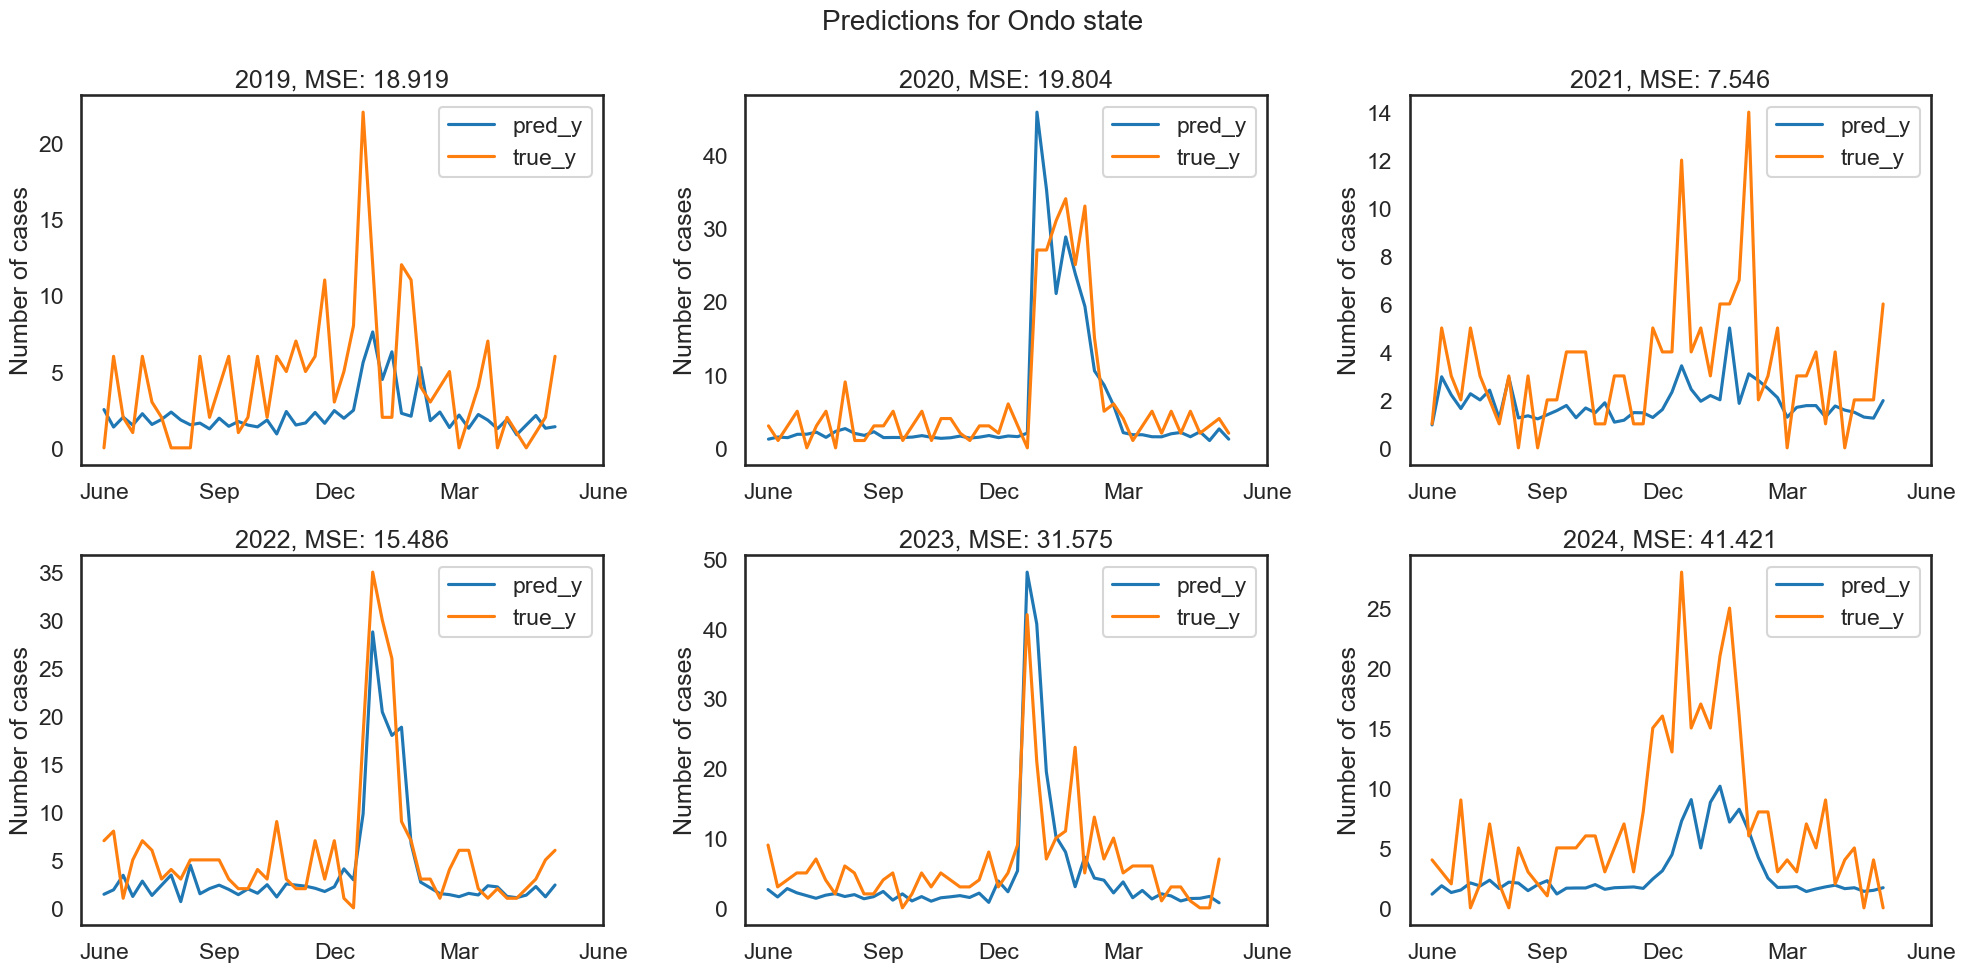
\includegraphics[width=\linewidth]{MAR_model_Per_State_One_Output/Ondo_mar_predictions.png}
\end{center}
\end{frame}

\subsubsection{Mar Model Per State Model Comparison}
%%%%%%%%%%%%%%%%%%%%%%%%%%%%%%%%%%%%%%%%%%%%%%%%%%%%%%%%%%%%%%%%%%%%%
% Per state Model Comparison
%%%%%%%%%%%%%%%%%%%%%%%%%%%%%%%%%%%%%%%%%%%%%%%%%%%%%%%%%%%%%%%%%%
% Bauchi
\begin{frame}{Per-State Model Comparison: All vs One – Bauchi Predictions}
\textbf{All vs One – Output: Bauchi Predictions}
\begin{center}
    \includegraphics[width=\linewidth]{MAR_model_Per_State_One_Output/Bauchi_All_vs_One_predictions.png}
\end{center}
\end{frame}
%
% Edo
\begin{frame}{Per-State Model Comparison: All vs One – Edo Predictions}
\textbf{All vs One – Output: Edo Predictions}
\begin{center}
    \includegraphics[width=\linewidth]{MAR_model_Per_State_One_Output/Edo_All_vs_One_predictions.png}
\end{center}
\end{frame}

% Ondo
\begin{frame}{Per-State Model Comparison: All vs One – Ondo Predictions}
\textbf{All vs One – Output: Ondo Predictions}
\begin{center}
    \includegraphics[width=\linewidth]{MAR_model_Per_State_One_Output/Ondo_All_vs_One_predictions.png}
\end{center}
\end{frame}



%%%%%%%%%%%%%%%%%%%%%%%%%%%%%%%%%%%%%%%%%%%%%%%%%%%%%%%%%%%%%%%%%%%%%
%%
%%\subsection{MAR Explainability}
%%\begin{frame}{MAR(4) Model: Explainability — Bauchi 2023}
%%\textbf{Violin Shap Plots and Feature Contribution Plot for Bauchi 2023}
%%\begin{center}
%%    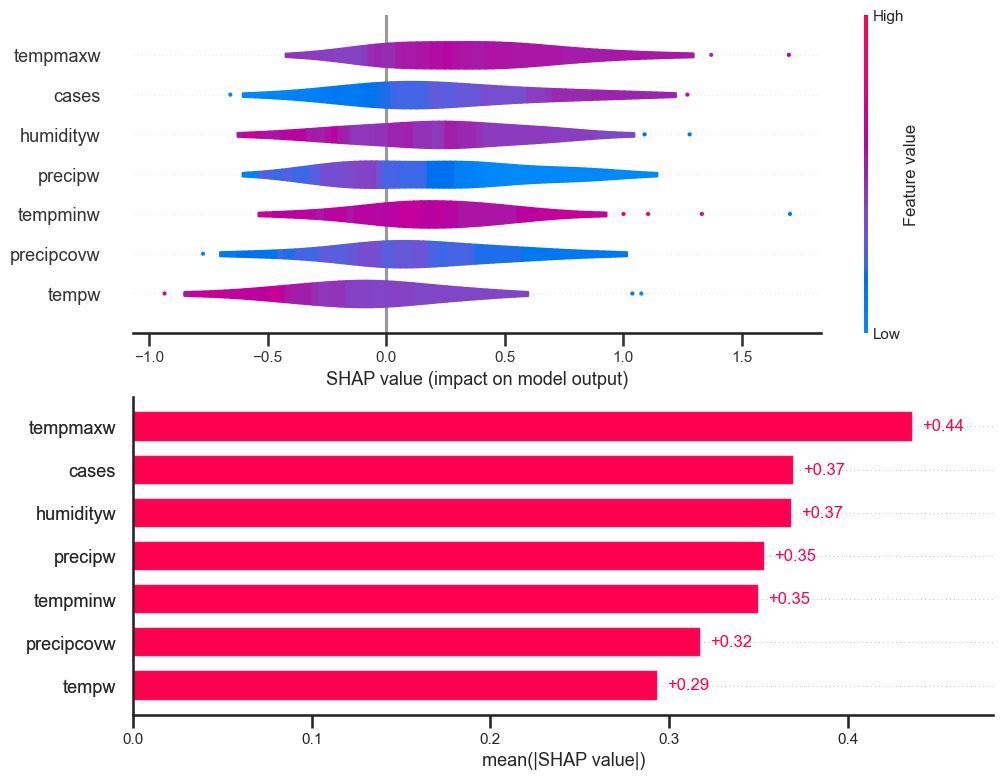
\includegraphics[width=\textwidth, height=0.85\textheight, keepaspectratio]{MAR_model/Bauchi_2023_MAR_model_explain.png}
%%\end{center}
%%\end{frame}
%%
%%\begin{frame}{MAR(4) Model: Explainability — Edo 2023}
%%\textbf{Violin Shap Plots and Feature Contribution Plot for Edo 2023}
%%\begin{center}
%%    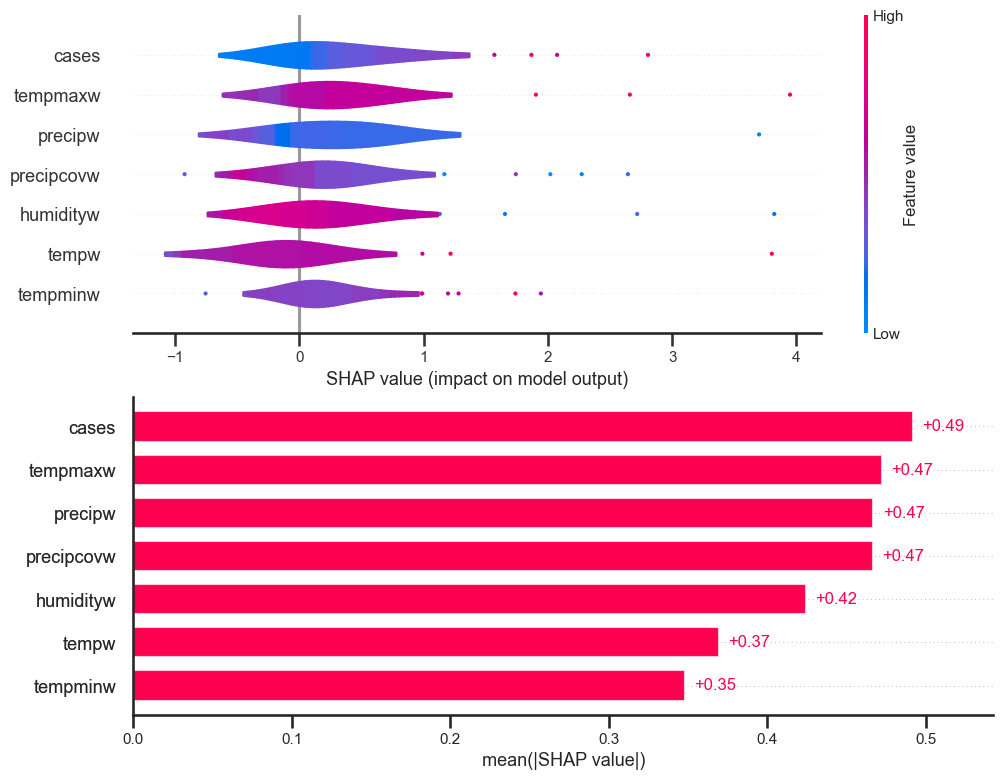
\includegraphics[width=\textwidth, height=0.85\textheight, keepaspectratio]{MAR_model/Edo_2023_MAR_model_explain.png}
%%\end{center}
%%\end{frame}
%%
%%\begin{frame}{MAR(4) Model: Explainability — Ondo 2023}
%%\textbf{Violin Shap Plots and Feature Contribution Plot for Ondo 2023}
%%\begin{center}
%%    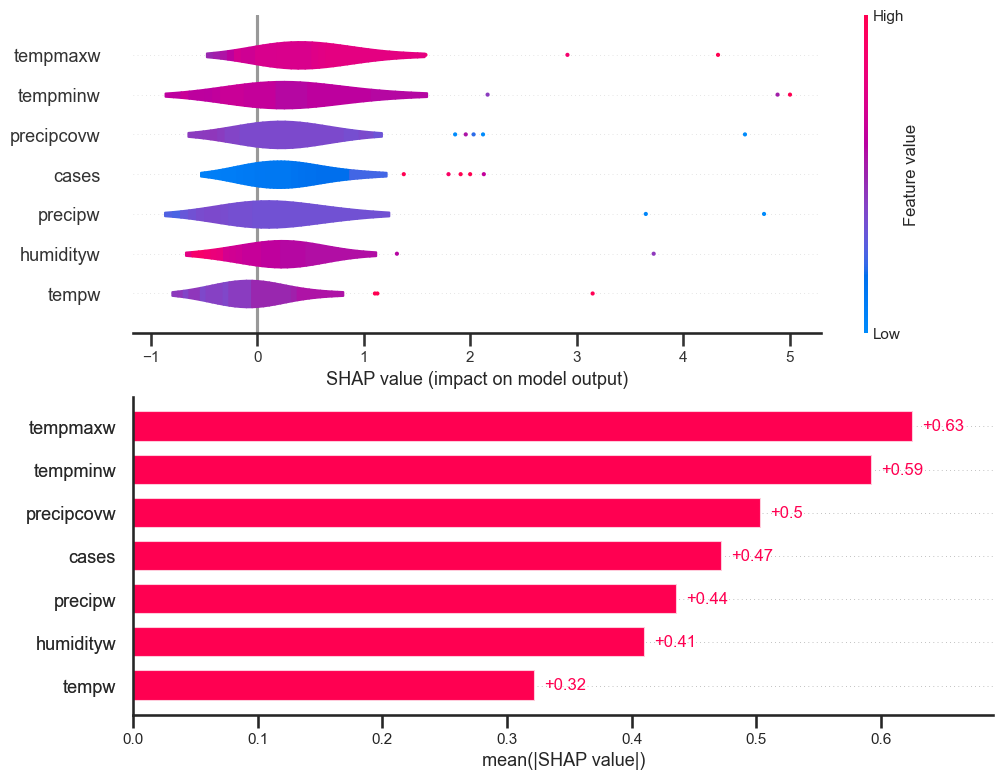
\includegraphics[width=\textwidth, height=0.85\textheight, keepaspectratio]{MAR_model/Ondo_2023_MAR_model_explain.png}
%%\end{center}
%%\end{frame}

\end{document}
